\documentclass[11pt]{article}
\newcommand{\HomeworkHeader}{习题一}
% Shared LaTeX preamble for homework/*/main.tex

% --- Base layout ---
\usepackage[a4paper, top=2.5cm, bottom=2.5cm, left=2cm, right=2cm]{geometry}
\usepackage{fontspec}
\usepackage[UTF8]{ctex}%latex支持中文宏包
\usepackage{amsmath, amssymb, amsthm}
\usepackage{mathtools}
\usepackage[svgnames]{xcolor}
\usepackage{pgfplots}
\pgfplotsset{compat=1.18}
\usepackage[most]{tcolorbox}
\usepackage{enumitem}
% Modified: Change label from hyphen (-) to bullet point ($\bullet$) for better visibility
\setlist[itemize]{label=$\bullet$}
\setlist[enumerate]{label=(\arabic*)}


% --- Colors ---
\definecolor{primaryColor}{RGB}{46, 52, 64}
\definecolor{accentColor}{RGB}{94, 129, 172}
\definecolor{boxFill}{RGB}{236, 240, 241}
\definecolor{solLine}{RGB}{163, 190, 140}
\definecolor{expandColor}{RGB}{191, 97, 106}

% --- TikZ styles (DFA / NFA / PDA) ---
\usepackage{tikz}
\usetikzlibrary{automata, positioning, arrows.meta, bending, backgrounds}
\tikzset{
    dfa_state/.style={
        state,
        thick,
        draw=accentColor,
        fill=boxFill,
        text=primaryColor,
        minimum size=1.1cm
    },
    dfa_edge/.style={
        ->,
        >=stealth,
        thick,
        draw=primaryColor,
        auto
    },
    pda_node/.style={
        state,
        thick,
        draw=accentColor,
        fill=boxFill,
        text=primaryColor,
        minimum size=1.2cm
    },
    pda_edge/.style={
        ->,
        >=stealth,
        thick,
        draw=primaryColor,
        auto
    },
    rule_expand/.style={
        pda_edge,
        draw=expandColor,
        text=expandColor
    },
    rule_match/.style={
        pda_edge,
        draw=solLine,
        text=solLine!80!black
    }
}

% --- Header / footer ---
\usepackage{fancyhdr}
\pagestyle{fancy}
\setlength{\headheight}{13.6pt}%避免页眉高度警告
\fancyhf{}
\fancyhead[L]{\kaishu 中国科学院大学}
\fancyhead[C]{林俊杰2023K8009916012}
\fancyhead[R]{\kaishu 理论计算机}
\usepackage{lastpage}
\cfoot{\small 第 \thepage \ 页，共 \pageref{LastPage} 页}

% --- Problem box ---
\newtcolorbox[use counter=problemSeq]{problem}[1][]{
    enhanced,
    breakable,
    colback=boxFill,
    colframe=accentColor,
    coltitle=white,
    fonttitle=\bfseries\large,
    title={题目 ~\theproblemSeq \quad #1},
    boxrule=0.5mm,
    arc=3mm,
    drop shadow=black!15!white,
    attach boxed title to top left={xshift=0.5cm, yshift*=-3mm},
    boxed title style={colback=accentColor},
    % 关键修改：每当创建一个新问题盒子时，自动将步骤计数器重置为0
    code={\setcounter{stepcount}{0}}
}

% --- Solution 环境 (红色盒子样式，支持可选序号) ---
% 修改说明：
% 1. [1][] 表示接受一个可选参数，默认为空
% 2. title={...} 中使用 \ifstrempty 判断是否有参数，如果有则添加空格和参数
\newtcolorbox{solution}[1][]{
    enhanced, breakable,
    colback=red!3!white,        % 背景色：淡粉
    colframe=red!75!black,      % 边框色：深红
    coltitle=white,
    fonttitle=\bfseries\Large\itshape,
    title={Solution\ifstrempty{#1}{}{~#1}}, % 动态标题：Solution (1)
    boxrule=0.5mm,
    arc=3mm,
    drop shadow=black!15!white,
    attach boxed title to top left={xshift=0.5cm, yshift*=-3mm},
    boxed title style={colback=red!75!black},
    before skip=0.5em,          % 盒子前的间距
    after skip=2em,             % 盒子后的间距
    before upper={\setcounter{stepcount}{0}} % 每个解答开始时重置步骤计数
}

% --- Title ---
\newcommand{\makeCustomTitle}[1]{
    \begin{center}
        \vspace*{1cm}
        {\Huge \bfseries \color{primaryColor} 作业 #1}\\
        \vspace{0.5cm}
        {\Large \color{accentColor} \today}
        \vspace{1.2cm}
    \end{center}
}

% --- 自定义环境定义 ---

% --- 自定义计数器与环境 ---
\newcounter{stepcount}
\newcounter{casecount}[stepcount]
\newcounter{problemSeq} % 新增：专门用于 Problem 的独立计数器

% 【关键修改】挂载钩子：每当遇到 \section 命令（含 \section*），将 problemSeq 计数器重置为 0
\pretocmd{\section}{\setcounter{problemSeq}{0}}{}{}

% 2. 定义带自动编号的步骤环境
\newenvironment{proofstep}[1]
  {%
    \refstepcounter{stepcount}% 增加计数
    \par\vspace{1.5em}%
    \noindent\textbf{\large \thestepcount. #1}% 输出 "1. 标题"
    \par\vspace{0.5em}%
  }
  {\par}

% 3. 定义无编号的结论环境 (用于最后的结论，格式同步骤)
\newenvironment{proofresult}[1]
  {%
    \par\vspace{1.5em}%
    \noindent\textbf{\large #1}% 仅输出标题
    \par\vspace{0.5em}%
  }
  {\par}

% 4. 定义带自动编号的情形环境
\newenvironment{proofcase}[1]
  {%
    \refstepcounter{casecount}% 增加计数
    \par\vspace{1em}%
    \noindent\textbf{情形 \thecasecount：#1}% 输出 "情形 1：标题"
    \par\vspace{0.2em}%
  }
  {\par}

\begin{document}
\makeCustomTitle{习题一}
% 来源：assets/习题一.pdf；第1页题2，第2页题4、7、10，第3页题15、16。
% 图1.7：原PDF第1页，裁剪区域(136,418,481,561) pt，6倍渲染，PNG无损保存。

\begin{problem}[原题 2：串联 RLC 电路的状态空间模型]
图 1.7 为电阻 $R$、电感 $L$、电容 $C$ 串联电路，输入为电源电压
$e(t)$，输出为电容电压 $V_C(t)$。以图示顺时针电流 $i(t)$ 和
$V_C(t)$ 为状态变量，建立状态方程及输出方程。
\begin{center}
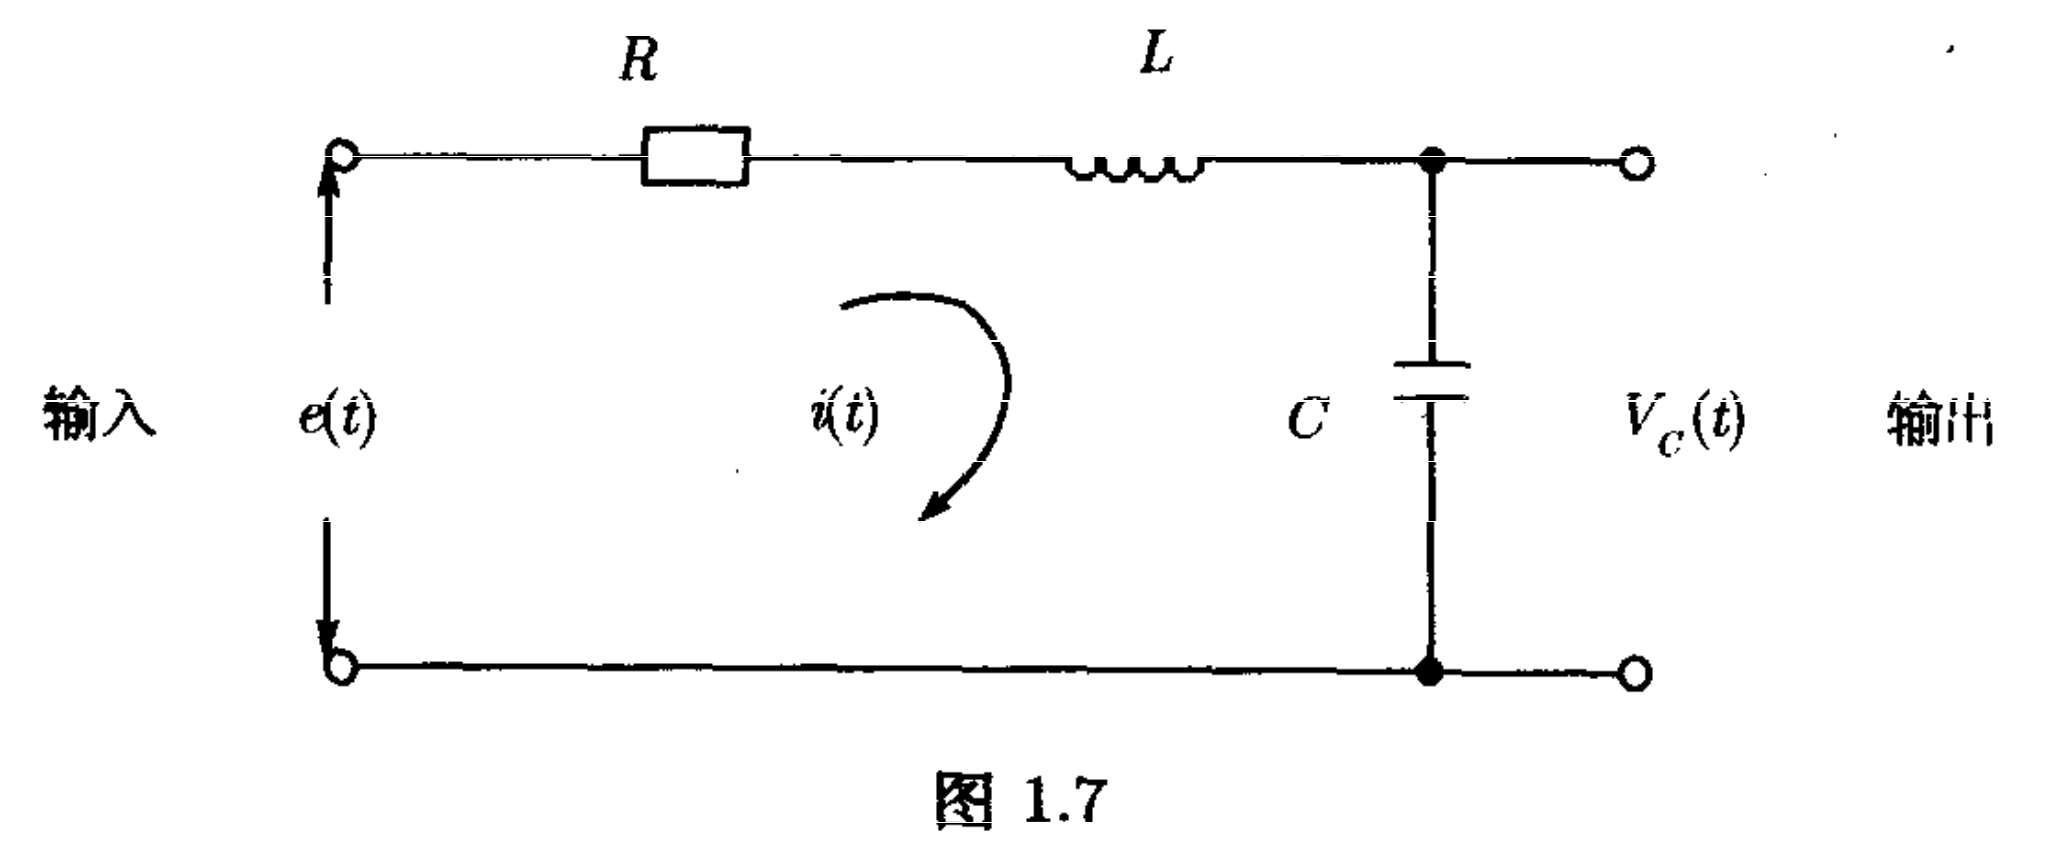
\includegraphics[width=0.88\linewidth]{figures/fig-1-7.png}
\end{center}
\end{problem}
\begin{solution}
\begin{proofstep}{确定状态、输入、输出及参考方向}
电感和电容是两个储能元件，可分别用电感电流和电容电压描述其储能状态。
按题意取
\[
x=\begin{bmatrix}x_1\\x_2\end{bmatrix}
=\begin{bmatrix}i\\V_C\end{bmatrix},\qquad u=e,\qquad y=V_C.
\]
沿图中的顺时针方向取电流为正，电容电压按上端相对下端取值。
这样电流流入电容的正端，电容采用关联参考方向。以下假设 $L>0,C>0$。
\end{proofstep}
\begin{proofstep}{利用电路定律写出两个一阶微分方程}
电阻、电感上的电压降分别为 $v_R=Ri$、$v_L=L\dot i$。
沿电流方向绕回路一周，由基尔霍夫电压定律，电源电压等于三个元件的电压降之和：
\[
e=Ri+L\dot i+V_C.
\]
移项并除以 $L$，得到
\[
\dot x_1=\dot i=-\frac RL x_1-\frac1L x_2+\frac1L u.
\]
由于各元件串联，流入电容的电流就是 $i$。由 $q=CV_C$ 及 $i=\dot q$，
\[
i=C\dot V_C,\qquad \dot x_2=\frac1C x_1.
\]
\end{proofstep}
\begin{proofstep}{整理状态方程与输出方程}
将两式中 $x_1,x_2,u$ 的系数按行排列，可得
\[
\boxed{\dot x=
 \begin{bmatrix}-R/L&-1/L\\1/C&0\end{bmatrix}x+
 \begin{bmatrix}1/L\\0\end{bmatrix}u,\qquad
 y=\begin{bmatrix}0&1\end{bmatrix}x.}
\]
输出直接取第二个状态，所以输出矩阵为 $[0\ 1]$，直接传递项 $D=0$。
\end{proofstep}
\begin{proofstep}{由输入输出方程核对模型}
由 $y=V_C$ 可知 $i=C\dot y$、$\dot i=C\ddot y$。代回电压定律得
\[
LC\ddot y+RC\dot y+y=u.
\]
零初始条件下，$Y(s)/U(s)=1/(LCs^2+RCs+1)$，与所列状态模型的
$C_y(sI-A)^{-1}B$ 相同。这里用 $C_y=[0\ 1]$ 表示输出矩阵，以区别电容参数 $C$。
\end{proofstep}
\end{solution}

\begin{problem}[原题 4：含输入导数的微分方程建模]
系统的输入输出关系为 $\ddot y-y=\dot u+u$。
引进状态变量，建立状态方程和输出方程。
\end{problem}
\begin{solution}
\begin{proofstep}{选择能够消去输入导数的状态}
若直接取 $x_1=y,x_2=\dot y$，第二个状态方程就会含有 $\dot u$。
标准状态方程希望只以 $u$ 作为外部输入。原方程中 $\ddot y$ 与 $\dot u$
恰好以 $\ddot y-\dot u$ 的形式出现，因此选择
\[
 x_1=y,\qquad x_2=\dot y-u.
\]
\end{proofstep}
\begin{proofstep}{逐项求导并写成矩阵形式}
根据第二个状态的定义，$\dot y=x_2+u$，于是
\[
\dot x_1=x_2+u.
\]
另一方面，由原方程 $\ddot y=y+\dot u+u$，
\[
\dot x_2=\ddot y-\dot u=(y+\dot u+u)-\dot u=x_1+u.
\]
两式合并，得到
\[
\boxed{\dot x=
\begin{bmatrix}0&1\\1&0\end{bmatrix}x+
\begin{bmatrix}1\\1\end{bmatrix}u,\qquad
y=\begin{bmatrix}1&0\end{bmatrix}x.}
\]
\end{proofstep}
\begin{proofstep}{确定初值对应关系，并验证与原方程等价}
给定 $y(0)$、$\dot y(0)$ 与 $u(0)$ 时，应取
$x(0)=[y(0),\ \dot y(0)-u(0)]^{\mathsf T}$。
反过来，由所建模型 $y=x_1$、$\dot y=x_2+u$ 可得
\[
\ddot y=\dot x_2+\dot u=x_1+u+\dot u=y+u+\dot u,
\]
即恢复原方程。因此模型既满足原微分方程，也保留了两个独立初始条件。
\end{proofstep}
\begin{proofstep}{说明传递函数约消与状态阶数的关系}
零初始条件下传递函数为
\[
G(s)=\frac{s+1}{s^2-1}=\frac{1}{s-1}.
\]
该约消仅描述零状态输入输出关系。一般初始条件下，原二阶方程仍可含
$e^{-t}$ 自由响应，故以上二阶状态模型保留了原方程的完整初始条件信息。
例如 $u=0$ 时，原方程有 $y=c_1e^t+c_2e^{-t}$；若仅用约消后的
一阶模型 $\dot y=y+u$，就无法保留任意 $c_2$ 对应的响应。
\end{proofstep}
\end{solution}

\begin{problem}[原题 7：由状态空间描述计算传递函数]
均有 $\dot x=Ax+Bu$、$y=Cx$，求 $G(s)$。
\begin{enumerate}
\item $A=\begin{bmatrix}0&1&0\\-2&-3&0\\-1&1&3\end{bmatrix}$，
$B=\begin{bmatrix}0\\1\\2\end{bmatrix}$，$C=\begin{bmatrix}0&0&1\end{bmatrix}$。
\item $A=\begin{bmatrix}0&1&0\\0&0&1\\-3&-1&-2\end{bmatrix}$，
$B=\begin{bmatrix}1&0\\0&1\\1&1\end{bmatrix}$，$C=\begin{bmatrix}1&1&1\end{bmatrix}$。
\end{enumerate}
\end{problem}
\begin{solution}
\begin{proofstep}{确定传递函数的计算条件与维数}
传递函数对应零初始条件，且本题均有 $D=0$，因此
$G(s)=C(sI-A)^{-1}B$。等价地，可以先对状态方程作拉普拉斯变换，
解出各 $X_i$ 与输入的关系，再用输出方程消去状态。
第（1）问的 $G$ 为标量；第（2）问有两个输入，$G$ 为 $1\times2$ 矩阵。
\end{proofstep}
\pagebreak
\begin{proofstep}{第（1）问：先求前两个状态，再求输出}
记状态的拉普拉斯变换为 $X_i$。零初值下，三个状态方程变为
\[
\begin{cases}
sX_1=X_2,\\
sX_2=-2X_1-3X_2+U,\\
sX_3=-X_1+X_2+3X_3+2U.
\end{cases}
\]
由第一式 $X_2=sX_1$，代入第二式得
$(s^2+3s+2)X_1=U$，所以
\[
X_1=\frac{U}{s^2+3s+2},\qquad X_2=sX_1.
\]
第三式整理为 $(s-3)X_3=(s-1)X_1+2U$。由于 $Y=X_3$，
\[
\frac YU=\frac1{s-3}\left(\frac{s-1}{s^2+3s+2}+2\right)
=\frac{s-1+2(s^2+3s+2)}{(s-3)(s^2+3s+2)}.
\]
通分、因式分解，最终得到
\[
\boxed{G(s)=\frac{2s^2+7s+3}{(s-3)(s+1)(s+2)}
=\frac{(2s+1)(s+3)}{(s-3)(s+1)(s+2)}.}
\]
\end{proofstep}
\begin{proofstep}{第（2）问：消元求解两个输入到状态的关系}
令输入为 $U=[U_1\ U_2]^{\mathsf T}$。由 $B$ 的各行可读出
\[
\begin{cases}
sX_1=X_2+U_1,\\
sX_2=X_3+U_2,\\
(s+2)X_3=-3X_1-X_2+U_1+U_2.
\end{cases}
\]
前两式依次给出
\[
X_2=sX_1-U_1,\qquad X_3=s^2X_1-sU_1-U_2.
\]
将这两式代入第三式，并将含 $X_1$ 的项移到左边，得到
\[
\underbrace{(s^3+2s^2+s+3)}_{d(s)}X_1
=(s^2+2s+2)U_1+(s+3)U_2.
\]
再代回 $X_2,X_3$，分别通分，便得
\[
\begin{bmatrix}X_1\\X_2\\X_3\end{bmatrix}=\frac{1}{d(s)}
\begin{bmatrix}
s^2+2s+2&s+3\\
s-3&s(s+3)\\
s(s-3)&s^2-s-3
\end{bmatrix}\begin{bmatrix}U_1\\U_2\end{bmatrix}.
\]
例如 $X_2$ 中 $U_1$ 的分子为
$s(s^2+2s+2)-d(s)=s-3$，其余各项同理由上述两条消元式得到。
\end{proofstep}
\pagebreak
\begin{proofstep}{第（2）问：利用输出方程合并各状态}
因为 $Y=X_1+X_2+X_3$，将上面矩阵每一列的三个分子相加：
\begin{align*}
U_1\text{ 的分子}&=(s^2+2s+2)+(s-3)+s(s-3)=2s^2-1,\\
U_2\text{ 的分子}&=(s+3)+s(s+3)+(s^2-s-3)=2s^2+3s.
\end{align*}
因此
\[
\boxed{G(s)=\frac{1}{s^3+2s^2+s+3}
\begin{bmatrix}2s^2-1&2s^2+3s\end{bmatrix}.}
\]
其中第一、第二个分量分别表示 $U_2=0$ 时 $Y/U_1$ 和 $U_1=0$ 时 $Y/U_2$。
\end{proofstep}
\end{solution}

\begin{problem}[原题 10：非零初始条件下的状态响应]
给定
\[
\dot x=\begin{bmatrix}0&1\\-2&-3\end{bmatrix}x+
\begin{bmatrix}2\\0\end{bmatrix}u,\quad
x(0)=\begin{bmatrix}0\\1\end{bmatrix},\quad u(t)=e^{-t},\ t\geq0.
\]
求 $x_1(t)$、$x_2(t)$。
\end{problem}
\begin{solution}
\begin{proofstep}{消去第二个状态，并换算初始条件}
由 $\dot x_1=x_2+2e^{-t}$ 可得 $x_2=\dot x_1-2e^{-t}$。
对第一个状态方程求导，再代入 $\dot x_2=-2x_1-3x_2$：
\begin{align*}
\ddot x_1&=\dot x_2-2e^{-t}\\
&=-2x_1-3(\dot x_1-2e^{-t})-2e^{-t}\\
&=-2x_1-3\dot x_1+4e^{-t}.
\end{align*}
注意二阶方程的初始导数是 $\dot x_1(0)=x_2(0)+2=3$，故
\[
\ddot x_1+3\dot x_1+2x_1=4e^{-t},\qquad
x_1(0)=0,\quad \dot x_1(0)=1+2=3.
\]
\end{proofstep}
\begin{proofstep}{求齐次解及受迫特解}
齐次特征方程为 $r^2+3r+2=(r+1)(r+2)=0$，所以齐次解为
$c_1e^{-t}+c_2e^{-2t}$。右端 $4e^{-t}$ 与齐次解中的 $e^{-t}$ 重合，
应将通常的待定系数形式再乘 $t$，设特解 $x_{1p}=at e^{-t}$。
有
\[
\dot x_{1p}=a(1-t)e^{-t},\qquad
\ddot x_{1p}=a(t-2)e^{-t}.
\]
代入微分方程左端得到
\[
a\bigl[(t-2)+3(1-t)+2t\bigr]e^{-t}=ae^{-t}=4e^{-t},
\]
因此 $a=4$，通解为
\[
x_1(t)=c_1e^{-t}+c_2e^{-2t}+4te^{-t}.
\]
\end{proofstep}
\begin{proofstep}{用初值确定常数，并恢复第二个状态}
将通解及其导数在 $t=0$ 处代入，得到
\[
\begin{cases}c_1+c_2=0,\\-c_1-2c_2+4=3.\end{cases}
\quad\Longrightarrow\quad c_1=-1,\ c_2=1.
\]
于是 $x_1=(4t-1)e^{-t}+e^{-2t}$。再用
\[
x_2=\dot x_1-2e^{-t}=(5-4t)e^{-t}-2e^{-2t}-2e^{-t},
\]
得到最终结果
\[
\boxed{\begin{aligned}
x_1(t)&=(4t-1)e^{-t}+e^{-2t},\\
x_2(t)&=(3-4t)e^{-t}-2e^{-2t},\qquad t\geq0.
\end{aligned}}
\]
\end{proofstep}
\begin{proofstep}{核对两个原状态方程}
所得解在 $t=0$ 时为 $x_1(0)=-1+1=0$、$x_2(0)=3-2=1$。
第一式已由 $x_2=\dot x_1-2e^{-t}$ 保证；第二式两边分别为
\begin{align*}
\dot x_2&=(4t-7)e^{-t}+4e^{-2t},\\
-2x_1-3x_2&=\bigl[-2(4t-1)-3(3-4t)\bigr]e^{-t}
 +(-2+6)e^{-2t}\\
&=(4t-7)e^{-t}+4e^{-2t}.
\end{align*}
故原状态方程和初始条件均满足。
\end{proofstep}
\end{solution}

\begin{problem}[原题 15：差分方程的离散状态空间模型]
给定
\[
y(k+2)+3y(k+1)+2y(k)=2u(k+1)+3u(k),
\]
写出离散动态方程。
\end{problem}
\begin{solution}
\begin{proofstep}{选择避免未来输入的状态变量}
二阶差分方程需要两个状态。若直接取 $y(k)$、$y(k+1)$，状态更新就会含有
$u(k+1)$。为使更新仅使用当前 $u(k)$，将原式中的
$y(k+2)-2u(k+1)$ 视为某个组合量在下一时刻的取值，定义
\[
x_1(k)=y(k),\qquad x_2(k)=y(k+1)-2u(k).
\]
\end{proofstep}
\begin{proofstep}{将状态定义向前移动一步}
第一式直接给出 $x_1(k+1)=y(k+1)=x_2(k)+2u(k)$。
第二式先利用原差分方程消去 $y(k+2)$，再用状态替换 $y(k),y(k+1)$：
\begin{align*}
x_1(k+1)&=x_2(k)+2u(k),\\
x_2(k+1)&=y(k+2)-2u(k+1)\\
&=-3y(k+1)-2y(k)+3u(k)\\
&=-2x_1(k)-3x_2(k)-3u(k).
\end{align*}
其中最后一步的输入系数为 $-3\times2+3=-3$。
\end{proofstep}
\begin{proofstep}{整理矩阵模型并说明初始化方式}
将当前状态和输入的系数按行排列，一组状态空间模型为
\[
\boxed{x(k+1)=\begin{bmatrix}0&1\\-2&-3\end{bmatrix}x(k)+
\begin{bmatrix}2\\-3\end{bmatrix}u(k),\qquad
y(k)=\begin{bmatrix}1&0\end{bmatrix}x(k).}
\]
这里 $x_2$ 是内部状态；其定义用于建立等价关系，实现时按上述递推式计算，
不需要提前测量下一时刻输出。初始条件对应为
$x(0)=[y(0),\ y(1)-2u(0)]^{\mathsf T}$。
由此初始化后，第一条递推式给出的 $y(1)$ 正好等于所指定的初始输出。
\end{proofstep}
\begin{proofstep}{消元核对原差分方程与脉冲传递函数}
由状态递推式有
\begin{align*}
y(k+2)&=x_2(k+1)+2u(k+1)\\
&=-2y(k)-3[y(k+1)-2u(k)]-3u(k)+2u(k+1)\\
&=-2y(k)-3y(k+1)+3u(k)+2u(k+1).
\end{align*}
将输出项移到左边，即回到题设差分方程。另一方面，
\[
zI-A_d=\begin{bmatrix}z&-1\\2&z+3\end{bmatrix},\qquad
(zI-A_d)^{-1}=\frac1{z^2+3z+2}\begin{bmatrix}z+3&1\\-2&z\end{bmatrix}.
\]
因此该模型的脉冲传递函数为
\[
G(z)=\begin{bmatrix}1&0\end{bmatrix}
\left(zI-\begin{bmatrix}0&1\\-2&-3\end{bmatrix}\right)^{-1}
\begin{bmatrix}2\\-3\end{bmatrix}
=\frac{2z+3}{z^2+3z+2},
\]
与原差分方程一致。
\end{proofstep}
\end{solution}

\begin{problem}[原题 16：连续系统的精确离散化]
给定
\[
\dot x=Ax+Bu,\qquad A=\begin{bmatrix}0&1\\0&0\end{bmatrix},\quad
B=\begin{bmatrix}0\\1\end{bmatrix},\quad T=2,
\]
求离散化状态方程。
\end{problem}
\begin{solution}
\begin{proofstep}{说明采样与保持方式，写出单个采样区间的状态解}
令 $x[k]=x(kT)$，采用零阶保持，即在 $[kT,(k+1)T)$ 上 $u(t)=u[k]$。
连续状态方程在该区间的解为
\[
x((k+1)T)=e^{AT}x(kT)
 +\int_{kT}^{(k+1)T}e^{A((k+1)T-t)}B\,u[k]\,dt.
\]
由于 $u[k]$ 在积分区间内为常量，将其提出；再作变量代换
$\tau=(k+1)T-t$，可得精确离散模型
\[
x[k+1]=Gx[k]+Hu[k],\qquad
G=e^{AT},\quad H=\int_0^T e^{A\tau}B\,d\tau.
\]
\end{proofstep}
\begin{proofstep}{计算状态转移矩阵}
直接相乘得
\[
A^2=\begin{bmatrix}0&1\\0&0\end{bmatrix}
\begin{bmatrix}0&1\\0&0\end{bmatrix}=0.
\]
因此矩阵指数级数中二阶及更高次项均为零：
\[
e^{A\tau}=I+A\tau+\frac{A^2\tau^2}{2!}+\cdots
=\begin{bmatrix}1&\tau\\0&1\end{bmatrix}.
\]
取 $\tau=T$，得到 $G=\begin{bmatrix}1&T\\0&1\end{bmatrix}$。
\end{proofstep}
\begin{proofstep}{积分计算输入矩阵}
先将状态转移矩阵乘以输入列向量：
\[
e^{A\tau}B=\begin{bmatrix}1&\tau\\0&1\end{bmatrix}
\begin{bmatrix}0\\1\end{bmatrix}=\begin{bmatrix}\tau\\1\end{bmatrix}.
\]
逐个分量积分，即有
\[
H=\int_0^T\begin{bmatrix}\tau\\1\end{bmatrix}d\tau
=\begin{bmatrix}T^2/2\\T\end{bmatrix}.
\]
这里 $A$ 为奇异矩阵，不能套用含 $A^{-1}$ 的公式；直接积分仍完全适用。
\end{proofstep}
\begin{proofstep}{代入采样周期并作物理核对}
取 $T=2$，最终得到
\[
\boxed{x[k+1]=\begin{bmatrix}1&2\\0&1\end{bmatrix}x[k]+
\begin{bmatrix}2\\2\end{bmatrix}u[k].}
\]
分量形式为
\[
x_1[k+1]=x_1[k]+2x_2[k]+2u[k],\qquad
x_2[k+1]=x_2[k]+2u[k].
\]
由原方程 $\dot x_2=u[k]$，长度为2的区间上 $x_2$ 增加 $2u[k]$；
再对 $\dot x_1=x_2$ 积分，增量为 $2x_2[k]+\tfrac12(2)^2u[k]$。
因此两个分量都与连续系统在恒定输入下的精确运动一致。
\end{proofstep}
\end{solution}
\end{document}
